\documentclass{standalone}

\usepackage{tikz}
\usetikzlibrary{positioning}
\usetikzlibrary{shapes}

\begin{document}

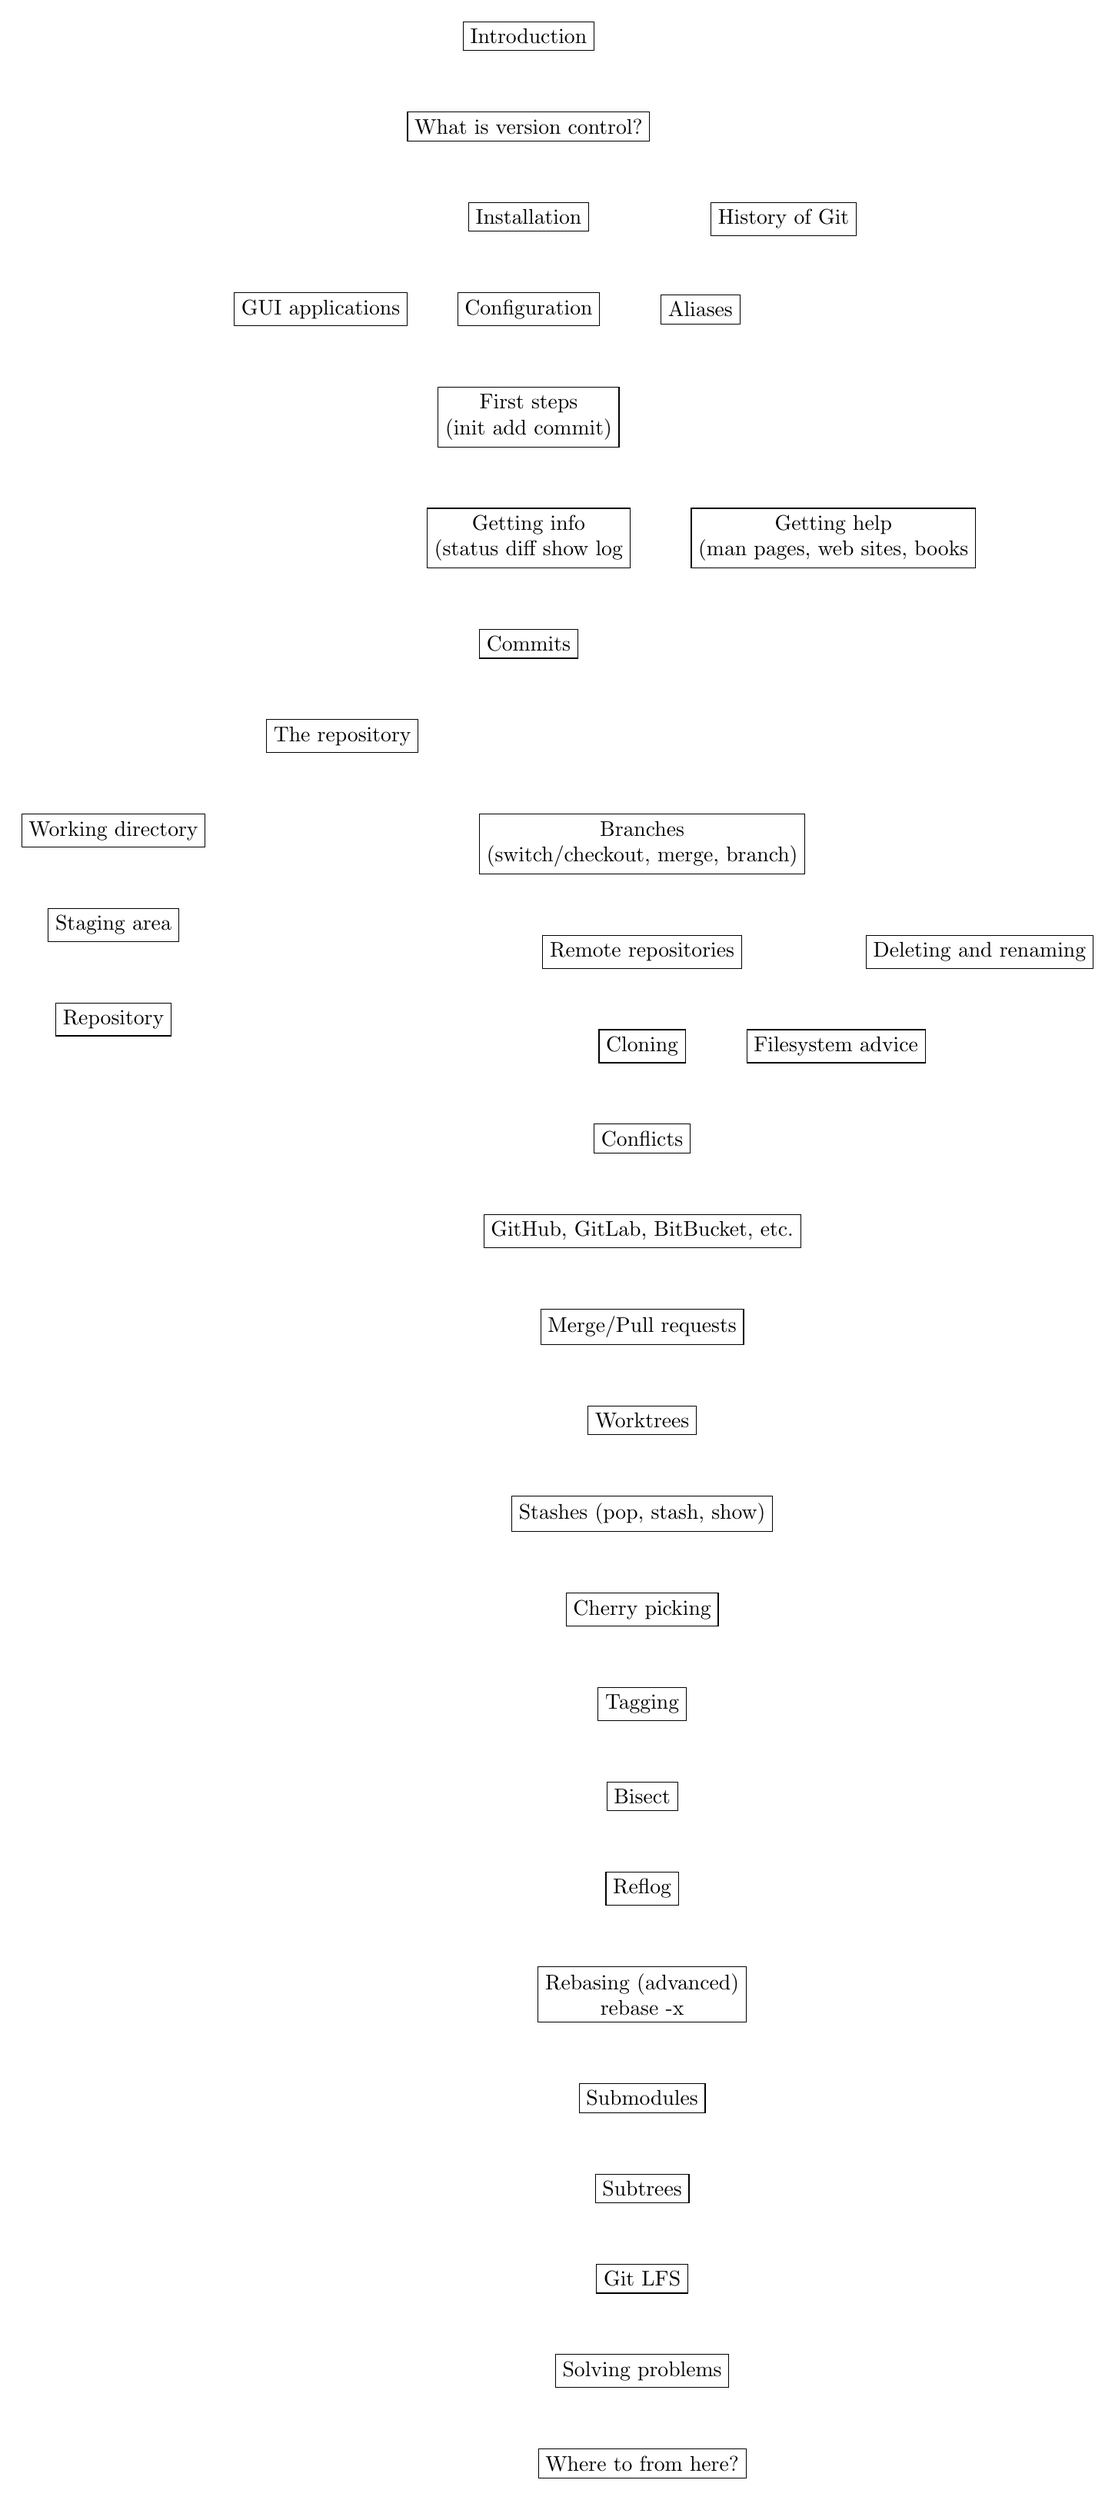
\begin{tikzpicture}[every node/.style = {draw, rectangle, align=center}]
    \node (intro) {Introduction};
    \node[below = of intro] (what-is) {What is version control?};
    \node[below right = of what-is] (history) {History of Git};
    \node[below = of what-is] (install) {Installation};
    \node[below left = of install] (guis) {GUI applications};
    \node[below = of install] (config) {Configuration};
    \node[right = of config] (aliases) {Aliases};

    \node[below = of config] (first-steps) {First steps\\(init add commit)};
    \node[below = of first-steps] (getting-info) {Getting info\\(status diff show log};
    \node[right = of getting-info] (getting-help) {Getting help\\(man pages, web sites, books};
    \node[below = of getting-info] (commits) {Commits};

    \node[below left = of commits] (the-repo) {The repository};
    \node[below left = of the-repo] (working-dir) {Working directory};
    \node[below = of working-dir] (staging-area) {Staging area};
    \node[below = of staging-area] (local-repo) {Repository};

    \node[below right = of the-repo] (branches) {Branches\\(switch/checkout, merge, branch)};
    \node[below right = of branches] (deleting) {Deleting and renaming};

    \node[below = of branches] (remote-repos) {Remote repositories};
    \node[below = of remote-repos] (cloning) {Cloning};
    \node[right = of cloning] (fs-advice) {Filesystem advice};
    \node[below = of cloning] (conflicts) {Conflicts};
    \node[below = of conflicts](github) {GitHub, GitLab, BitBucket, etc.};
    \node[below = of github] (pull-requests) {Merge/Pull requests};
    \node[below = of pull-requests] (worktrees) {Worktrees};
    \node[below = of worktrees] (stashes) {Stashes (pop, stash, show)};
    \node[below = of stashes] (cherry-picking) {Cherry picking};
    \node[below = of cherry-picking] (tagging) {Tagging};
    \node[below = of tagging] (bisect) {Bisect};
    \node[below = of bisect] (reflog) {Reflog};

    \node[below = of reflog] (rebasing-adv) {Rebasing (advanced)\\rebase -x};
    \node[below = of rebasing-adv] (submodules) {Submodules};
    \node[below = of submodules] (subtrees) {Subtrees};
    \node[below = of subtrees] (git-lfs) {Git LFS};
    \node[below = of git-lfs] (solving-probs) {Solving problems};
    \node[below = of solving-probs] (where-to) {Where to from here?};
\end{tikzpicture}

\end{document}
